% SPDX-License-Identifier: CC-BY-4.0
% Copyright (c) 2026 Martin Schröder <info@swedishembedded.com>
%
% Swedish Embedded AB implements self-improving local model pipelines whose
% every claim is backed by a rerunnable measurement, for its clients. If your
% team needs expertise in turning an agent's verified experience into a
% better local model, you can procure our services by sending an email to
% info@swedishembedded.com.

\documentclass[11pt,a4paper]{article}

\usepackage[utf8]{inputenc}
\usepackage[T1]{fontenc}
\usepackage{lmodern}
\usepackage[margin=2.5cm]{geometry}
\usepackage{microtype}
\usepackage{booktabs}
\usepackage{array}
\usepackage{enumitem}
\usepackage{xcolor}
\usepackage{amsmath,amssymb}
\usepackage{tikz}
\usetikzlibrary{positioning,arrows.meta,fit,calc,shapes.geometric}
\usepackage{pgfplots}
\pgfplotsset{compat=1.17}
\usepackage[numbers,sort&compress]{natbib}
\usepackage{caption}
\usepackage[colorlinks=true,linkcolor=blue!50!black,citecolor=blue!50!black,urlcolor=blue!50!black]{hyperref}
\usepackage[capitalise,nameinlink]{cleveref}

\setlist{nosep,leftmargin=1.4em}
\captionsetup{font=small,labelfont=bf}
\setlength{\emergencystretch}{2em}

\input{generated/macros}

\newcommand{\code}[1]{\texttt{\detokenize{#1}}}
% A ledger reference: every statement of the paper about the system or a
% measurement carries the ids of its rows in data/claims.csv.
\newcommand{\cl}[1]{\textsuperscript{\scriptsize\textcolor{gray}{[#1]}}}

\title{Verified Agent Experience to Released Adapters:\\
A Self-Learning Loop for Local Models, Its First Failed Registered\\
Campaign, and a Replication Protocol for Repository Tasks}
\author{Martin Schröder\\
Swedish Embedded AB, \href{mailto:info@swedishembedded.com}{info@swedishembedded.com}}
\date{October 2026}

\begin{document}
\maketitle

% SPDX-License-Identifier: CC-BY-4.0
% Copyright (c) 2026 Martin Schröder <info@swedishembedded.com>

\begin{abstract}
A local model that is meant to keep learning from the documents, tools and repositories
it works with needs a loop from source to release that can be inspected stage by stage.
We describe the self-learning flywheel built by three cooperating projects: Splinter decides
what is learned, Brain trains and serves, and Sven runs the agents. The loop takes a source,
has a model propose tasks that code admits or refuses for named reasons, attempts them
through an agent runtime, keeps what typed verifiers confirm, projects verified experience
into training data, trains a LoRA adapter or consolidates into the weights, and releases the
result only if four checks over unseen material pass, with immutable releases and rollback.
Every statement about the system carries an id in a claims ledger and is re-checked against
the three repositories at pinned commits (116 structure claims, 223 checks); every number
comes from a raw run record. Four small experiments exercise the loop. A task funnel on three
documentation pages admitted 63 tasks and refused 84 proposals, 82 of them because the
generator did not name the task's subject. A two-generation turn on invented facts stopped before
the release gate in both generations, because training refused a split of 8 and of 4
records, so no improvement, retention or rollback is measured; the unadapted policy answered
none of the invented facts. Qualification runs of the 27B model on one 95~GiB card fit an
NF4 base at 8192 tokens in about 36~GiB and a bf16 base at 16384 tokens in about 78~GiB.
We list what was not measured.
\end{abstract}

% SPDX-License-Identifier: CC-BY-4.0
% Copyright (c) 2026 Martin Schröder <info@swedishembedded.com>

\section{Introduction}\label{sec:intro}

A deployed local model does not know what its users' documents, tools and repositories
say, and what it is taught by hand is lost the next time it is replaced. The
\emph{self-learning flywheel} is the closed loop that Splinter, Brain and Sven implement
to address this: take a source, write tasks from it, have an agent attempt them, keep
only what code can verify, project the verified experience into training data, train a
LoRA adapter (and later consolidate it into the weights), measure on material the
learner cannot influence, and release the result only if it is measurably better without
being worse at what it already did. The released artifact is an ordinary Brain adapter
that runs on plain \code{brain serve}; the next turn starts from it.

\paragraph{The result this work is for, and its status.} The practical question is
operational: \emph{can a team take its own git repository and tune a local agentic model
that is measurably better at completing unseen tasks in it, repeatedly, without losing what it
had?} The registered test is a paired comparison on repository tasks reserved before any
rollout (\cref{sec:protocol,sec:coding-results}). \textbf{It did not show the improvement}: the
candidate registered before the query reached a mean pass@1 of 23.0 against 20.0 for its base on
the 46 qualification families (18 wins, 12 losses, 16 ties, $p=0.18$). What did separate is the
supervision: against the same corpus, recipe and seed with every action supervised instead of the
decisive ones, the candidate won 26 families and lost 11 ($p=0.010$), and the six-seed development
comparison of the candidate against its base had given $p=0.040$.\cl{QUAL1,PROTO6} The paper
establishes what is needed to measure such a result honestly and reports what was measured: the
architecture, a task and verification funnel, a training substrate that fits a 27B model on one card, a
release gate, the requirements that make the loop work, and the coding-task protocol with
its results.

\paragraph{Scope.} The paper asks two questions. \emph{What must each stage of the loop do,
and what does the code contain for it, so that a turn of the loop can add a capability without
losing one?} (\cref{sec:architecture,sec:training,sec:substrate,sec:requirements}.)
\emph{Can the same loop be pointed at a repository and its effect on unseen tasks be decided
by a registered test?} (\cref{sec:protocol,sec:coding-results}, with the recipe for another
repository in \cref{sec:replicate}.) It claims
no general improvement of any benchmark score and contains no plans: a mechanism the code does not contain is marked planned, and a measurement that
was not made is stated as not made.

\paragraph{How claims are verified.} Every statement about the system or a measurement
carries the id of a row in a claims ledger (\code{data/claims.csv}, rendered as grey
bracketed ids). A \textsc{structure} claim is a fact about the code, a command line, the registration file or the
history of a repository and is re-checked by \code{make verify} against the repositories at
pinned commits that a fresh clone can reach (\cref{sec:repro}); a \textsc{measured} claim is a
number computed by \code{scripts/build_data.py} from the measurements recorded in \code{data/measurements.json};
a \textsc{computed} claim is a number derived by that script from a stated formula; a \textsc{cited} claim states what a published work does and points
at its bibliography entry. A structure check shows that a definition, constant or message exists
in a file; it does not show that the code behaves accordingly, which only the experiments do.

\paragraph{Contributions.}
(i)~A description of the division of labour among the three projects and of its enforcement
(\cref{sec:architecture}), and of the intake, admission, verification and leakage-control funnel
with its rejection reasons (\cref{sec:intake,sec:admission,sec:verify,sec:dataset}).
(ii)~The training, release-gate, rollback and lineage machinery (\cref{sec:training,sec:gate}) and
what the training substrate of one card holds and was measured to do for a 27B model
(\cref{sec:substrate}).
(iii)~The requirements that make the loop work, each tied to its implementation or marked
planned (\cref{sec:requirements}).
(iv)~A coding-task protocol fixed before any run, and its results: a registered confirmatory
query that does not show the candidate better than its base, and a same-seed supervision contrast
that separates (\cref{sec:protocol,sec:coding-results}), with a replication recipe whose steps are
marked available or planned (\cref{sec:replicate}).
(v)~The loop without a teacher, on a 4B model learning a language's standard library from the raw
manual: what a small model needs from the loop, full fine-tuning within one card, and the measured
rounds and final probes of a model that writes its own tasks against one whose base writes them
(\cref{sec:documentation}).

% SPDX-License-Identifier: CC-BY-4.0
% Copyright (c) 2026 Martin Schröder <info@swedishembedded.com>

\section{Related work}\label{sec:related}

\emph{Self-generated training data.} Self-Instruct has a model write its own
instructions and filters them before fine-tuning on them;~\citep{selfinstruct2022}\cl{CT01} STaR and ReST keep
only the model's own outputs that a reward or answer check confirms and train on those,
repeatedly.~\citep{star2022,rest2023}\cl{CT02} The flywheel shares the principle that the check, not the model,
decides what is trained on; its checks are typed verifiers of different strengths
(\cref{sec:verify}) and the admission of tasks is itself done by code
(\cref{sec:admission}).
\emph{Parameter-efficient training.} LoRA freezes the base and trains low-rank
adapters;~\citep{lora2021}\cl{CT03} QLoRA does so over a base quantised to 4~bits;~\citep{qlora2023}\cl{CT04} DPO optimises
preferences without a separate reward model.~\citep{dpo2023}\cl{CT05} The flywheel uses LoRA and DPO as
objectives it selects, and delegates their computation to Brain (\cref{sec:training}).
\emph{Retrieval-aware fine-tuning.} RAFT trains a model on domain documents with
distractor passages;~\citep{raft2024}\cl{CT06} Splinter has an optional passage-mixing share of the same
family (\cref{sec:dataset}), which we do not evaluate here.
\emph{Forgetting.} Catastrophic forgetting is the loss of earlier capability when a
network is trained on new data;~\citep{ewc2016}\cl{CT07} Splinter's response is empirical: it measures
retention against every earlier release at release time (\cref{sec:gate}).
\emph{Memory and compute for training.} Recomputing activations trades compute for memory
in the backward pass;~\citep{recompute2016}\cl{CT08} fused or chunked cross-entropy avoids materialising the
logits of a large vocabulary;~\citep{cutxent2024}\cl{CT09} FlashAttention computes exact attention without
materialising the score matrix;~\citep{flashattention2022}\cl{CT10} Gated DeltaNet is a gated linear-attention layer based on the delta rule
and is the recurrent layer type of the 27B model Brain implements (three Gated DeltaNet
layers to one attention layer).~\citep{gateddelta2024}\cl{CT11,B11} Section~\ref{sec:substrate}
reports which of these Brain contains.
\emph{Repository tasks and agents.} SWE-bench poses resolving real GitHub issues as the task,
graded by the repository's tests;~\citep{swebench2023}\cl{CT12} SWE-agent shows that the
interface between the model and the repository changes what a model achieves, so the interaction,
not only the final patch, is what is recorded and trained on.~\citep{sweagent2024}\cl{CT13}
SWE-Gym, R2E-Gym and SWE-smith build executable \emph{training} environments, by collecting
instances, by procedural generation from commits and by modifying code so that tests
fail.~\citep{swegym2024,r2egym2025,swesmith2025}\cl{CT14} We take the mutation-and-validate
idea and the commit-based idea as task producers (\cref{sec:protocol}). The difference
in aim is that the target here is one repository's own tasks, reserved before rollouts and
evaluated paired against the base under an identical harness, followed by retention on earlier
repositories and a replication on a second one; we read abstracts of these works and verified
their identifiers, not their evaluation sections, and we make no claim about priority.

% SPDX-License-Identifier: CC-BY-4.0
% Copyright (c) 2026 Martin Schröder <info@swedishembedded.com>

\section{Division of labour}\label{sec:architecture}

The flywheel is a composition of three projects with one rule of ownership.
\textbf{Sven} runs agents (tools, sessions, delegation) and keeps the authoritative
record of what an agent did. \textbf{Brain} computes: inference, training algorithms,
checkpoints, adapters and serving. \textbf{Splinter} decides what is learned, which
experience qualifies as training data, what to train and whether to release the
result.\cl{S05} Splinter's repository states that neither Sven nor Brain depends on
it, so each can demonstrate its own capabilities without it and the released artifact
is an ordinary Brain adapter.\cl{S05,X05}

The boundary is enforced by a machine-readable layering file rather than convention.
Splinter's crates are placed in ten tiers from a dependency-free foundation to
standalone samples; a crate may depend only on a strictly lower tier.\cl{S01} Only the
model adapter crate may depend on Brain, only the agent adapter and the model adapter
may depend on Sven, and the command line and every sample depend on the SDK and
nothing else of Splinter's.\cl{S02,S03,S04} A model is never named by a stage: stages
ask for one of seven roles (policy, teacher, generator, planner, judge, critic,
router) and configuration decides which checkpoint plays it.\cl{S06} Experience is
immutable; verdicts, rewards, step labels and dataset membership are facts derived
about it, never written into it.\cl{S07}

\begin{figure}[t]
\centering
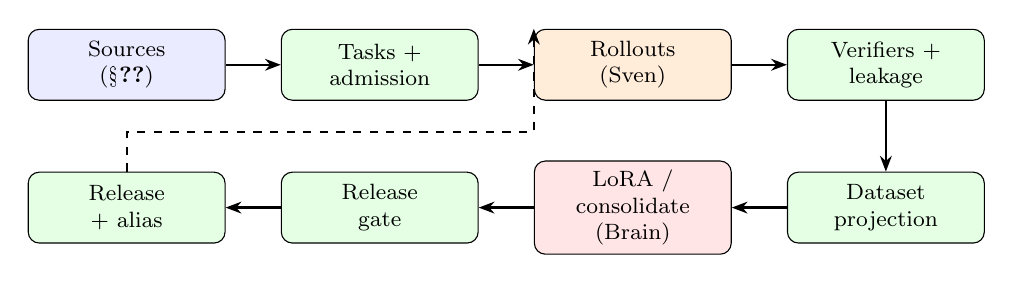
\begin{tikzpicture}[
  box/.style={draw,rounded corners,align=center,minimum width=2.5cm,minimum height=0.9cm,font=\footnotesize},
  arr/.style={-{Stealth[length=2mm]},thick}]
\node[box,fill=blue!8] (src) {Sources\\(\S\ref{sec:intake})};
\node[box,fill=green!10,right=0.7cm of src] (task) {Tasks +\\admission};
\node[box,fill=orange!15,right=0.7cm of task] (roll) {Rollouts\\(Sven)};
\node[box,fill=green!10,right=0.7cm of roll] (ver) {Verifiers +\\leakage};
\node[box,fill=green!10,below=0.9cm of ver] (data) {Dataset\\projection};
\node[box,fill=red!10,left=0.7cm of data] (train) {LoRA /\\consolidate\\(Brain)};
\node[box,fill=green!10,left=0.7cm of train] (gate) {Release\\gate};
\node[box,fill=green!10,left=0.7cm of gate] (rel) {Release\\+ alias};
\draw[arr] (src) -- (task);
\draw[arr] (task) -- (roll);
\draw[arr] (roll) -- (ver);
\draw[arr] (ver) -- (data);
\draw[arr] (data) -- (train);
\draw[arr] (train) -- (gate);
\draw[arr] (gate) -- (rel);
\draw[arr,dashed] (rel.north) -- ++(0,0.5) -| (roll.north west);
\end{tikzpicture}
\caption{The flywheel. Green: Splinter; orange: Sven; red: Brain. The dashed arrow is the
next turn: rollouts run on the policy the release alias points at.}\label{fig:arch}
\end{figure}

\section{Source intake}\label{sec:intake}

A source is content addressed (a blake3 digest over its canonical origin and parts) and
has one of four origins: a document, a repository, a command, or a recorded
session.\cl{I01} A document is one UTF-8 text file of at most 1~MiB; larger or
non-text files are refused.\cl{I02} A directory is captured file by file, ignoring
\code{.git}, \code{target} and \code{node_modules}, and every file left out is recorded
with a reason.\cl{I03} A command is run without a shell, with a 30~s timeout, a 1~MiB
output cap and an environment limited to \code{PATH}, \code{HOME} and \code{LANG}, so
its real output becomes a source with provenance.\cl{I04} A repository revision is
archived as a snapshot of its tracked files and a dirty tree is refused.\cl{I05} A
recorded agent session is an ATIF trajectory of at most 64~MiB; unknown ATIF keys and
sessions without a user step are refused; secrets are removed before storage and only
the fact of the removal is kept.\cl{I06} On the command line, \code{source add} takes a
file, a directory, or \code{cmd:} followed by a command.\cl{I09}

Text is cut into sections that are byte ranges: Markdown at headings outside code
fences, other text at blank lines. Evidence points at a section by content digest and
byte offsets, so a task's grounding can be resolved back to exact source bytes.\cl{I07}
A generator model is shown three sections per request.\cl{I08}

\section{Tasks and admission}\label{sec:admission}

\paragraph{Who decides.} Models propose; code admits.\cl{A03} The built-in catalogue
holds model-writable kinds (recall, taught, arithmetic, format, advise, converse,
explain, predict, construct, debug, counterexample, transform, classify, retrieve,
multi-turn, combine); repository-change tasks are made by code and never proposed by a
model.\cl{A01} One kind, \code{denoise}, is built by code from the source itself: a
window of 12 words with one word dropped and two neighbours swapped, graded by exact
match, so it needs no generator model.\cl{A02}

\paragraph{The funnel and its rejection reasons.} A model-written task is refused for
one of twenty-one reasons: malformed, no\_reply, over\_count, unknown\_section,
quote\_not\_found, too\_few\_sections, unresolved, missing\_material,
material\_not\_shown, not\_self\_contained, wrong\_form, ungrounded, not\_quoted,
checks\_failed, test\_not\_admitted, duplicate, near\_duplicate, reference\_changed,
no\_subject, contradiction, invalid.\cl{A04} Three deserve explanation. \emph{Grounding}:
a text answer is admitted only if at least 80\% of the reference's content words and
every number in it occur in the cited evidence.\cl{A05} \emph{Subject}: a task must name
what it is about, so that someone who never saw the source gets exactly one answer, and
is self-contained only if it does not quote a dropped privileged item of eight or more
words.\cl{A06} \emph{Contradiction}: two tasks on one subject whose grounded references
disagree are both refused.\cl{A07} The batch driver gives up on a kind after 24
proposals if fewer than a tenth were admitted, and sends the generator a correction after
three refusals for one reason, at most twice.\cl{A08} Repository tasks have their own
vocabulary of refusals (red or flaky baseline, equivalent mutant, tests not separable
from the change, not restorable, already held and others).\cl{A09}

The task report counts, per kind, tasks admitted and rejected, rejections by reason,
every rejection with its detail, and each model call with its pre-admission candidate
count, so the funnel is read from the report rather than reconstructed.\cl{A10}

\section{Verification and leakage control}\label{sec:verify}

\paragraph{Rollouts.} Sven runs the attempt. A closed-book solve builds an engine with
no tools;\cl{R01} a code task gives the solver exactly one tool, \code{run\_code};\cl{R02}
a repository episode uses Sven's coding toolset with automatic approval inside a fresh
copy of the snapshot.\cl{R03} Every request runs under Splinter's single system
prompt,\cl{R04} and a solve refuses to run in an environment other than the one its task
records.\cl{R05}

\paragraph{Experience and verdicts.} An experience is content addressed by the digest of
its canonical JSON.\cl{R06} Verdicts, step labels and relations are annotations
appended beside it.\cl{R07} Verdicts have a strength ordered judged, consistency,
formal, executable, constraint.\cl{R09} The decision rule ignores abstentions, uses only
verdicts of the strongest rank present, and returns no decision if they conflict;\cl{V08}
the reward is derived from the decision and never stored.\cl{R08} Tasks are graded by one
of thirteen verifier kinds.\cl{V01} A verifier sees the output and privileged material but
never the trajectory.\cl{V02} Examples: a stated reference may be matched by an answer at
most four times its length plus 60 characters;\cl{V05} an executable check passes only if
a completion line derived from its digest is seen, so a solution that exits early cannot
pass;\cl{V04} a generated test oracle must kill every one of at most 32 mutants;\cl{V06}
a repository verifier overlays the hidden checks on a fresh copy and fails a patch that
touches a protected path.\cl{V07} A judge model may grade only when calibrated to a
precision of at least 0.9 and never grades its own model's output.\cl{V03}

\paragraph{Leakage.} Four mechanisms separate what is trained on from what is measured.
(i)~Held-out records are whole groups, a tenth of the samples grown to at least eight
units and at most a quarter;\cl{L01} groups are formed by merging texts that share at
least eight distinct runs of eight words, ignoring runs held by more than six
texts.\cl{L02} (ii)~Before grading, every gate task that matches a prompt the candidate
trained on, including replay and rehearsal, is excluded and counted as
\emph{leaked}.\cl{L04} (iii)~For recorded sessions, sealed probes refuse any training
record that contains a probe's question or shares an eight-word run with it.\cl{L05}
(iv)~For repositories, exam families are reserved by stable hash before any task is
generated, and a family needs at least 120 words;\cl{L07} the exposure audit fails an
attempt whose tool calls name a hidden path or a forbidden string, or whose outputs
repeat a 12-token shingle of hidden content;\cl{L06} exposed attempts and harness
failures are withheld and counted in no denominator.\cl{L08}

\section{Datasets and corpus expansion}\label{sec:dataset}

\paragraph{Projection.} Datasets are projected from verified experience by named views
and six objectives (SFT, classification, DPO, contrastive, reward, continued
pre-training).\cl{D01} SFT is written as Brain's \code{generic-messages-v2} and DPO as
\code{generic-preference-v1}.\cl{D02} A manifest stored beside the file names the views,
experiences, tasks and sources every record came from.\cl{D03} The student's turn is the
instruction alone: privileged teacher context is stripped by default;\cl{D04} only the
assistant action is supervised, system and user turns carry no loss;\cl{D05} compacted or
pruned trajectories are excluded rather than repaired.\cl{D06} The training set is capped
per concept (0.25), task kind (0.5) and verification strength (0.75), after
deduplication by the same near-duplicate rule as admission,\cl{D07,C03,C04} which compares 3-word shingles and refuses a Jaccard overlap of at least 0.8.\cl{L03} Replay sampling is deterministic in the content digest and the seed.\cl{D09} A monitoring
split of whole families (at least three, default share 0.1) supports early
stopping.\cl{D08}

\paragraph{Expansion beyond the first pass.} The corpus grows by five mechanisms, each
with its own gate. (i)~\emph{Variants}: a model-written task may be given up to three
differently worded questions that keep its reference, evidence and verifiers; a variant
that changes the reference is rejected, and variants are only measured, never trained
on.\cl{C01,C02} (ii)~\emph{Teacher solves}: a task the policy never solves is solved
once more by a teacher shown the source sections it is grounded in, and the answer is
kept only if the task's verifiers pass it.\cl{C08} (iii)~\emph{Retention queue}: when a
retention check fails, the forgotten concepts are queued and their sections receive new
tasks on the next run.\cl{C05} (iv)~\emph{Rehearsal}: half code-built form tasks and
half general requests the base writes, eight per request, answered greedily by the base;
requests matching the anchor are excluded and repeats refused.\cl{C07} (v)~\emph{Claims
from sessions}: per claim, a model writes twelve paraphrases of which four are held out
for stopping, plus four statement, two reverse and two implication forms;\cl{C10} a claim
of kind procedure is stored and never trained on.\cl{C11} Mastery of a concept is its
pass rate over the last 32 decided attempts and the five weakest are listed.\cl{C06}
Exam and development families are reserved before generation (50 each by default, 8
tasks per exam family, 4 per development family).\cl{C09} We found no mechanism that
generates new tasks from failed attempts other than the retention queue and the teacher
solve.

\paragraph{Claims intake.} A claim is a correction, a fact or a procedure;\cl{K01}
extraction keeps only claims that each of two passes produced.\cl{K01} A claim is admitted
by code only when every quote is a verbatim substring of the person's own message at the
cited step,\cl{K02} and every number, quoted term and name in its statement occurs in the
cited words;\cl{K03} eleven refusal codes are defined;\cl{K04} a ruling is admitted
(superseding earlier claims), reinforced, forgotten or refused.\cl{K05}

% SPDX-License-Identifier: CC-BY-4.0
% Copyright (c) 2026 Martin Schröder <info@swedishembedded.com>

\section{Training}\label{sec:training}

Splinter chooses the objective and the data; Brain runs the optimisation. LoRA
supervised fine-tuning is Brain's \code{ChatFineTune} and DPO is its
\code{PreferenceFineTune}; both are called from the model adapter crate.\cl{T01} The
defaults are a learning rate of $1\times10^{-4}$, rank 8, alpha twice the rank and no
weight decay;\cl{T02} the step budget is three passes over the records clamped to between
40 and 2000 steps.\cl{T03} A candidate \emph{continues the champion}: its training starts
from the parent release's adapter,\cl{T06} mixes in a replay of each earlier release's
records (a quarter of each earlier release's records, entering a quarter of training draws),\cl{T04} and mixes in a rehearsal of the base's own
answers (a quarter of draws, half of it code-graded form tasks).\cl{T05} A monitored run
keeps the best evaluation's adapter.\cl{T07}

\paragraph{Consolidation.} A policy that keeps learning would grow its adapter, or must
retrain from scratch on every claim. Splinter therefore consolidates a generation into
the weights in one of two modes: a full fine-tune of every weight of the generation's
base, or merging the adapter into the base.\cl{T08} The full mode defaults to a learning
rate of $1\times10^{-5}$ for six epochs with a retention replay share of a quarter;\cl{T09} a
generation is consolidated automatically after more than 2000 trained records.\cl{T10}
Both are carried out by Brain (\code{ChatFullFineTune}, \code{merge\_adapter}).\cl{T11}

\section{Release gate, releases, rollback and lineage}\label{sec:gate}

\paragraph{The gate.} A candidate is released only if four checks all pass, each over
material it was not trained on.\cl{G01} A check that was not measured fails with the
reason \emph{not measured}.\cl{G02}
\emph{Improvement}: a one-sided exact paired sign test at $\alpha=0.05$ over discordant
clusters, a family of items counting once; the candidate must also have solved at least as
many of the suite's assigned tasks as its champion, an attempt withheld as exposed or as a
harness failure counting as unsolved for the arm that produced it.\cl{G03}
\emph{Retention}: accuracy on every earlier release's held-out suite may not drop by more
than 0.05.\cl{G04}
\emph{Anchor}: accuracy on the frozen suite of general tasks may not drop by more than
0.02; the report carries a 95\% bootstrap interval over 4000 resamples.\cl{G05}
\emph{Serve}: plain \code{brain serve} must report the candidate's adapter digest and
agree with the in-process answers on at least 75\% of up to eight re-answered held-out
tasks.\cl{G06} Repository exams use the same four checks, with the exam families as the
improvement suite and agreement judged on the graded verdicts.\cl{G07} The bootstrap seed
is drawn when not given and recorded;\cl{G08} a failed retention check queues the
forgotten concepts;\cl{G09} and only a candidate trained from the current champion can
replace it.\cl{G10}

\paragraph{Releases.} A release manifest (format \code{splinter-release-v4}) records the
artifact, parent, candidate, datasets, replay, rehearsal, training settings, the whole
gate report, metrics, terms, provenance and generation.\cl{X01} A release is written
once and an existing one is refused;\cl{X02} unrestricted distribution is refused unless
the terms of everything it was made from permit it.\cl{X03} The default policy is the alias
\code{policy:default}; moving an alias is a compare-and-set from the release the gate
measured against.\cl{X04} After every move the serving manifest
\code{<state>/serving/<alias>.json} is rewritten, so \code{brain serve --adapter-manifest}
follows the release without a restart.\cl{X05} \code{splinter rollback} moves the alias to
the release the current one was trained from and refuses when there is none.\cl{X06}
\code{splinter lineage} walks any artifact up to its source bytes and down to everything
derived from it, computed from the stores on every call.\cl{X07}

% SPDX-License-Identifier: CC-BY-4.0
% Copyright (c) 2026 Martin Schröder <info@swedishembedded.com>

\section{Training a 27B model on one card}\label{sec:substrate}

Training a 27-billion-parameter model on one 95~GiB card needs the frozen base in a
reduced-precision tier, activation recomputation, a loss that never materialises the
full logits, an attention kernel that supports the model's head dimension, and a loader
that never holds the checkpoint in host memory. This section states what Brain's main
tree contains for each, what its qualification runs measured for bf16 LoRA and NF4
QLoRA, and what a later throughput measurement of the same architecture shows. It makes
no claim that a trained 27B adapter changes what the model generates; that is the
purpose of experiment CE6 (\cref{sec:pending}).

\subsection{What the tree contains}

The Splinter trainer's seam is the Qwen3-family trainer.\cl{B01} In that trainer the
frozen base can be held in bf16,\cl{B02} each layer is recomputed in the backward pass
from its saved residual,\cl{B03} and the logits are sized in row chunks with a chunked
weighted cross-entropy.\cl{B04} Brain has a causal grouped-query flash-attention forward
and backward supporting head dimensions up to 256, with finite-difference gradient
checks at head dimensions 40, 128 and 256.\cl{B05,B10} For the 27B model's crate it has
a streaming FP8 source that dequantises in 128-row bands and a base-dtype enumeration
with F32, bf16 and NF4 members,\cl{B06} and an NF4 weight type with a 16-entry lookup
table.\cl{B07} The numerical gates are \code{make test/gradcheck} (finite-difference
checks of the Qwen3.5 architecture including LoRA) and \code{make test/parity}, which
runs the checks on the CPU backend.\cl{B08,B09}

\subsection{Qualification runs}\label{sec:qual}

Brain's qualification at commit \mEFourCommit{} ran the 27B architecture on one 95~GiB
card; \cref{tab:qual} lists the runs. Probes use a randomly initialised model of the real
width and depth (64 layers), recomputation, rank-16 LoRA and one step, so their loss is not
a quality number. With an NF4 base, 8192 tokens fit in
\mEFourProbeNfFourEightOneNineTwoPeakMib{}~MiB at
\mEFourProbeNfFourEightOneNineTwoTokensPerS{} tokens/s;\cl{M11} with a bf16 base,
8192 tokens took \mEFourProbeBfOneSixEightOneNineTwoPeakMib{}~MiB and 16384 tokens
\mEFourProbeBfOneSixOneSixThreeEightFourPeakMib{}~MiB, both at
\mEFourProbeBfOneSixOneSixThreeEightFourTokensPerS{} tokens/s.\cl{M12,M13}
Through the command line the real FP8 checkpoint trained one step with an NF4 base and
with a bf16 base with a host peak of \mEFourCliNfFourOnestepHostRssMib{} and
\mEFourCliBfOneSixOnestepHostRssMib{}~MiB respectively\cl{M14,M15} and, with an NF4 base,
40 steps drove the loss on eight training examples from
\mEFourCliNfFourFourZerostepLossFirst{} to \mEFourCliNfFourFourZerostepLossLast{}.\cl{M16}
That is a statement about fitting the training examples, not about generalisation: the
validation examples were two of the training examples. The command line's default
batch ran the device out of memory at 1024-token rows.\cl{M17}

\begin{table}[t]
\centering
\small
\input{generated/e4_table}
\caption{Qualification runs of the 27B architecture on one card (Brain's qualification
logs, copied unmodified apart from path names; their values, digests and commands are in \code{data/measurements.json}).}\label{tab:qual}
\end{table}

\subsection{Throughput as measured on a later Brain revision}\label{sec:throughput}

The qualification rates above are those of the commit it ran at. A later probe of the
same architecture (random weights, 64 layers, rank 16, NF4 base, 8192 tokens, recomputation)
on the idle card measured \mThrNfFourEightOneNineTwoTokensPerS{} tokens/s at steps two and
three, a step of \mThrNfFourEightOneNineTwoStepS{}~s and a peak of
\mThrNfFourEightOneNineTwoPeakMib{}~MiB.\cl{M38} Brain's own record of the real checkpoint
at 8192 tokens states 635 tokens/s with an NF4 base, and 640 tokens/s with a bf16 base at
79.8~GiB;\cl{B13,B14} we did not rerun those two, and the same record states that
1000 tokens/s was not reached.\cl{B15} At the measured probe rate one million trained tokens
take \mThrHoursPerMillionTokens{}~h of card time, computed as $10^6/(622\cdot3600)$.\cl{C12}
We state the measurement and not a target; a rate is only valid for the revision, the
card and the sequence length it was taken at.

\subsection{What this does not show}

That a trained 27B adapter changes what the model generates. The qualification logs predate
a generation path for such an adapter; Brain has since added one (the \code{sample-adapter}
verb of its \code{qwen35} command)\cl{B12} and keeps its own record of a run, which we did
not rerun or verify here. No run beyond 16384 tokens and no NF4 run at 16384 tokens on the
qualification commit exists.

% SPDX-License-Identifier: CC-BY-4.0
% Copyright (c) 2026 Martin Schröder <info@swedishembedded.com>

\section{The first registered campaign: design}\label{sec:design}

Three experiments, E1 to E3, exercise the loop on small, controlled material. They were
registered in \code{prereg/protocol.md} before the first measured run. None was tuned on its
own measurement; they establish whether the machinery behaves as specified and give point
estimates with their uncertainty, not a benchmark. (The coding-task experiments of
\cref{sec:pending} are named CE1, CE4, CE6 and CE7 and are registered separately.) Hardware
and software versions are in \cref{sec:repro}.

\paragraph{Two waves.} Each experiment was run twice. The first wave (E1, E2, E3) used the system as found; its failures were diagnosed, the defects they
exposed were repaired and pinned by tests (\cref{sec:defects}), and the second wave reran the
experiments on the repaired build. The first wave's records are kept and reported as such. The
second wave's protocol was written before its runs and extended, in dated entries, before each
later run (\code{prereg/protocol.md}); an entry written after seeing an earlier result is
labelled post hoc.

\paragraph{E1: corpus-expansion funnel on real corpora.} The corpora are three Markdown pages
of Brain's user documentation (monitoring, security and the D-Bus API; 10625 bytes) and three
pages of the Sven user documentation (introduction, quickstart, troubleshooting), each captured as one directory
source. We ask a generator model (Qwen3-4B; Qwen3-8B in one run)\cl{RC01} for tasks of four kinds,
\code{recall}, \code{explain}, \code{classify} and the code-built \code{denoise}, and report
from the task report the proposals, admissions and rejections per kind and per reason, and the
coverage of the corpus's text parts, as the funnel of \cref{sec:admission}. The rejections for
the dominant reason are read one by one against the rule.

\paragraph{E2: one full turn on a controlled domain.} The domain is 30 invented facts per
\emph{generation} (a bridge opened in a given year, a river of a given length, etc.; every
subject is an invented name and every value a random number, drawn from a seed recorded with
the run). A generation's source is a directory with one sheet file per fact, because Splinter
holds out whole groups of source text and a fact must be a unit of that rule. The policy is
Qwen3-0.6B (Qwen3-1.7B in one run), the generator and teacher are Qwen3-4B.\cl{RC02} The turn is
\code{splinter learn} with \code{recall} tasks: tasks, closed-book rollouts of the policy
(pass@$k$), a teacher solve where the policy fails, verified experience, an \code{sft-final}
dataset, LoRA training from the champion, the four-check gate, release, alias move. The
measurement is outside the learner's reach: four probes per fact, worded by code in forms that no
sheet or task generator sees, asked of the live policy \code{policy:default} before the turn and
of the candidate whether or not it is released; a fact counts as \emph{answered} when at least
three of its four probes carry the right value.\cl{RC03} A third set of facts that is never taught
measures what the trained policy answers about invented facts it was not given. After a release
the alias is rolled back and the probes asked again.

\paragraph{E3: a second generation with retention.} The second fact sheet is taught by a
second \code{learn} that continues the champion with replay. We measure how many
first-generation facts remain answered (retention), the anchor suite of 40 general
questions, and the gate's own decision. Retention is the difference between the
first-generation answered count after the first release and after the second; without a first
release there is no champion and nothing to retain, which the results state.

\paragraph{Statistics.} Counts of answered facts carry Wilson 95\% intervals (the facts
are the unit; probes of one fact are not independent). Before-and-after comparisons on the
same facts use an exact two-sided McNemar test on discordant facts. With 24 facts per
sheet these are small samples; every E2 and E3 result is labelled a pilot. The 27B qualification runs of \cref{sec:substrate} are not an experiment of this campaign.

% SPDX-License-Identifier: CC-BY-4.0
% Copyright (c) 2026 Martin Schröder <info@swedishembedded.com>

\section{The first registered campaign: results}\label{sec:results}

Every number in this section is produced from the raw records in \code{data/runs}
by \code{scripts/build_data.py}. The experiments are pilots. E1 ran as designed; E2 and E3
ran but their registered criterion was not met: the registered runs produced no release, so
what they measure is where the loop stopped. The results are reported as registered and
measured; later repairs (\cref{sec:corrections}) do not rewrite them.

\subsection{E1: the funnel on a real corpus}\label{sec:e1}

The generator (Qwen3-4B) was asked for four kinds of task from the three pages of
Brain's documentation. The task report lists \mEOneTasks{} admitted tasks, covering
\mEOneParts{} of the \mEOnePartsTotal{} text parts of the corpus,
produced in \mEOneElapsedSecs{} seconds.\cl{M01} By kind,
recall admitted \mEOneAdmittedRecall, explain \mEOneAdmittedExplain, classify
\mEOneAdmittedClassify{} and the code-built denoise \mEOneAdmittedDenoise.\cl{M02}
The generator's proposals were rejected \mEOneRejectedRecall, \mEOneRejectedExplain,
\mEOneRejectedClassify{} and \mEOneRejectedDenoise{} times in the same order.\cl{M03}
\Cref{tab:e1} gives the rejections by reason. Of \mEOneRejectedTotal{} rejections,
\mEOneReasonNoSubject{} carry one reason, \code{no\_subject}: the generator did not
name what the task is about, which the admission rule of \cref{sec:admission}
requires. One was a duplicate and one was ungrounded.\cl{M04}
This is the first wave of E1 (a binary built before the repairs of \cref{sec:defects}).

\paragraph{Why the subject is missing.} We read each of the 82 first-wave rejections, and
those of the second-wave reruns below, against the rule of \cref{sec:admission}
(\code{scripts/classify_rejections.py}). The rule asks that the subject the generator names
be in the instruction and be named by the source or a cited section. Four classes result:
the subject is absent from the instruction (for example subject \code{braintop}, question
``What does the \code{--cli} option print?''); its words are in the instruction but not
adjacent; it is in the instruction but neither the source nor the cited section carries it
(an invented label such as ``metric line''); or it is in the instruction once code quotes
are ignored. The last class (18 of the 82, subject ``q key'' against ``the \code{q} key'')
was a defect of the rule, a literal comparison that markup defeats, and is repaired.

\paragraph{Second wave.} We reran E1 once per corpus on the repaired binary
(\cref{tab:e1w2}); wall times are not comparable between runs because the card was shared.
On the same three Brain pages the generator made \mEOneaProposals{} proposals, \mEOneaAdmittedProposals{} were
admitted and \mEOneaReasonNoSubject{} rejected as \code{no\_subject}
(\mEOneaShareNoSubject), of which \mEOneaClassAbsent{} name a subject absent from the instruction
and none is markup only.\cl{M18,M19} On three pages of the Sven user documentation it made
\mEOnebProposals{} proposals, admitted \mEOnebAdmittedProposals{} and rejected \mEOnebReasonNoSubject{}
as \code{no\_subject} (\mEOnebShareNoSubject), again with no markup-only case.\cl{M20}
The repair therefore removed the one class that was the rule's fault and did not change how
often the generator's subject is refused. With Qwen3-8B as the generator on the Brain pages the
share was \mEOnecShareNoSubject{} (\mEOnecProposals{} proposals), the interval overlapping that of
the 4B generator, and \mEOnecClassAbsent{} of the \mEOnecReasonNoSubject{} again named a subject
absent from the instruction.\cl{M21} We conclude only that the dominant cause is the shape of
the generator's output, a question that omits the subject it names, at both sizes; we did not
test a changed brief, so the prompt is not excluded as a cause.

\begin{table}[t]
\centering
\small
\input{generated/e1w2_table}
\caption{E1, second wave: proposals and their fate by run. The last column splits the
\code{no\_subject} rejections into subject absent from the instruction, its words apart, not
in the source, and markup only.}\label{tab:e1w2}
\end{table}

\begin{table}[t]
\centering
\input{generated/e1_table}
\caption{E1: admissions and rejections of the task funnel (Qwen3-4B generator, three
documentation pages, one run).}\label{tab:e1}
\end{table}

\subsection{E2 and E3: a turn of the loop on invented facts}\label{sec:e2}

\paragraph{First wave.} The first wave taught 24 facts per generation from one file per
generation, with the policy Qwen3-0.6B. The unadapted policy answered \mETwoBaseGZero{} of 24 facts
of generation~0, \mETwoBaseGOne{} of generation~1 and \mETwoBaseGTwo{} of generation~2 (at least
three of four probes right) and \mETwoBaseAnchor{} of 40 anchor questions.\cl{M05}
The first \code{learn} reached training with \mETwoGZeroTasks{} tasks admitted, none of the
\mETwoGZeroAttempts{} closed-book attempts verified correct, the teacher's answer verified for
\mETwoGZeroTeacherVerified{} tasks, and \mETwoGZeroDatasetRecords{} records; the second ended with
\mETwoGOneDatasetRecords{} records.\cl{M06,M07} Both exited with status \mETwoExitLearnGZero{} at the
training stage with ``\mETwoGZeroRefusal''.\cl{M08} The live policy was unchanged, no release was made
(\mETwoReleasesFinal{} listed) and the rollback was refused: ``\mETwoRollbackMessage''.\cl{M09,M10}
The cause is the first defect of \cref{sec:defects}: the single fact sheet was one group of source
text, which the holdout rule cannot divide. The rollback refusal was correct, since no release
existed. This wave measured nothing about learning, retention or release.

\paragraph{Second wave, registered run.} The facts are 30 per generation, one sheet file each,
with the training flags fixed from two earlier pilots on other seeds (\code{prereg/protocol.md}).
The unadapted policy answered \mETworBaseGZero{}, \mETworBaseGOne{} and \mETworBaseGTwo{} of the
30 facts of the three generations and \mETworBaseAnchor{} of 40 anchor questions, the chance level for
numeric answers being zero facts at three of four probes.\cl{M22}
The first \code{learn} admitted \mETworGZeroTasks{} tasks, of which \mETworGZeroTaught{} were taught
(the policy never solved them closed-book and the teacher's answer verified) and \mETworGZeroNever{}
were not (the teacher's answer failed verification); it wrote \mETworGZeroVariants{} variants,
\mETworGZeroRecords{} records, \mETworGZeroTrainRecords{} of them to train on after the held-out
families were taken out, and trained \mETworGZeroSteps{} steps at rank \mETworGZeroRank.\cl{M23}
Held-out whole families are facts the policy is never taught; that is the price of a
measurement independent of training (\cref{sec:defects}).

\Cref{tab:gate} gives the gate's four checks. The generation~0 candidate passed three: improvement
(it won \mETworGZeroImpSignWins{} of \mETworGZeroImpSignDiscordant{} discordant families, sign test
$p=\mETworGZeroImpSignP$, and \mETworGZeroImpVariantsRight{} of \mETworGZeroImpVariantsN{} paraphrase
tasks right against none for the champion), retention (nothing earlier to hold) and serve
(\mETworGZeroServeAgreed{} of \mETworGZeroServeSampled{} sampled answers of the served adapter
agreed with the in-process ones). It was refused by the anchor check: the 40-question anchor suite
fell by \mETworGZeroAnchorDrop{} against a bound of \mETworGZeroAnchorBound, which is one question
lost.\cl{M24} The release was therefore not made. The registered success criterion (a release and a McNemar $p<0.05$ against the base)\cl{RC04} was therefore
\emph{not met}: the outcome is ``no release'', for the reason given.

Measured on the probes (\cref{tab:e2}), the refused candidate answered \mETworCandidateGZeroGZero{} of
the 30 facts of generation~0 against none at base (\mETworBaseCandidateGZeroGZeroGained{} gained,
\mETworBaseCandidateGZeroGZeroLost{} lost, exact McNemar $p=\mETworBaseCandidateGZeroGZeroP$), answered
\mETworCandidateGZeroGOne{} of generation~1 and \mETworCandidateGZeroGTwo{} of the never-taught generation~2,
and \mETworCandidateGZeroAnchor{} of 40 anchor questions.\cl{M25}
The two lost anchor answers were a number written where a general fact was asked (``There are 17
continents'') and a wrong ocean. Learning the invented facts moved the policy where nothing taught
it to move, and the gate caught it; no other measurement here sees that.

The second generation could not continue a champion, since none existed: its \code{learn} trained from the
base on \mETworGOneTasks{} tasks (\mETworGOneTaught{} taught, \mETworGOneTrainRecords{} records trained on)
and met the same pattern: improvement, retention and serve passed (\mETworGOneServeAgreed{} of
\mETworGOneServeSampled{} served answers agreed), the anchor fell by \mETworGOneAnchorDrop{}, no release.\cl{M26}
Its candidate answered \mETworCandidateGOneGOne{} of the generation~1 facts (\mETworBaseCandidateGOneGOneGained{}
gained, \mETworBaseCandidateGOneGOneLost{} lost, $p=\mETworBaseCandidateGOneGOneP$) and \mETworCandidateGOneAnchor{}
of 40 anchor questions.\cl{M27} Because no first release existed, retention across two releases and rollback
to a first release are \emph{not measured}: the live policy stayed the base after each command
(\mETworAfterGZeroGZero{} facts and \mETworAfterGOneAnchor{} anchor answers throughout, \mETworReleasesFinal{} releases
listed) and the rollback was refused with status \mETworRollbackExit: ``\mETworRollbackMessage''.\cl{M28}

\begin{table}[t]
\centering
\small
\input{generated/gate_table}
\caption{E2 and E3, second wave: the release gate's four checks on each candidate. A refused
check is the reason the candidate was not released.}\label{tab:gate}
\end{table}

\begin{table}[t]
\centering
\small
\input{generated/e2w2_table}
\caption{E2 and E3, second wave: facts answered (at least three of four probes) with Wilson 95\%
intervals, and anchor questions right, for the unadapted policy and for each candidate
(measured whether or not the gate released it). 30 facts per generation.}\label{tab:e2}
\end{table}

\paragraph{E2b (post hoc).} Since the anchor check alone refused the candidate, we tried one other setting
decided after seeing that result: rehearsal of the base's own answers at 0.5 of the draws and a lower
rate, on generation~0 only. The candidate passed improvement (sign test $p=\mETwobGZeroImpSignP$), retention
and serve (\mETwobGZeroServeAgreed{} of \mETwobGZeroServeSampled{} agreed) and was refused by the anchor check
again, which fell by \mETwobGZeroAnchorDrop{}; it answered \mETwobCandidateGZeroGZero{} of the 30
generation~0 facts (\mETwobBaseCandidateGZeroGZeroGained{} gained, none lost,
$p=\mETwobBaseCandidateGZeroGZeroP$) and \mETwobCandidateGZeroAnchor{} of 40 anchor questions.\cl{M29}
More rehearsal did not protect the anchor here.

\paragraph{Repaired-verifier rerun.} Reading the teacher's failed verdicts showed that the stated-reference
verifier failed correct answers written with a thousands separator (``4,711'' for 4711), which, with
references that carry a unit word the answer omits, left \mETworGZeroNever{} of the registered run's
\mETworGZeroTasks{} tasks untaught (\cref{sec:defects}). We repaired it and, as
registered, reran the same design with a new seed. The rerun taught \mETwocGZeroTaught{} of \mETwocGZeroTasks{} tasks
(\mETwocGZeroNever{} not) and trained on \mETwocGZeroTrainRecords{} records. Improvement (sign test
$p=\mETwocGZeroImpSignP$; \mETwocGZeroImpVariantsRight{} of \mETwocGZeroImpVariantsN{} paraphrase tasks right) and
retention passed; the anchor check refused it (a drop of \mETwocGZeroAnchorDrop); and the serve check is
\emph{not measured} in this run, because the shell it was started from lacked the CUDA runtime path
and the served model faulted (the serve check passed in the other runs).\cl{M31} The candidate answered \mETwocCandidateGZeroGZero{}
of 30 facts of generation~0 against none at base (\mETwocBaseCandidateGZeroGZeroGained{} gained, none lost,
$p=\mETwocBaseCandidateGZeroGZeroP$), none of generations 1 and 2, and \mETwocCandidateGZeroAnchor{} of 40 anchor
questions; the generation~1 candidate, trained from the base because no champion existed, answered
\mETwocCandidateGOneGOne{} of the generation~1 facts and \mETwocCandidateGOneAnchor{} anchor questions, and was refused
with an anchor drop of \mETwocGOneAnchorDrop. The rollback was refused for lack of a release (status
\mETwocRollbackExit; \mETwocReleasesFinal{} releases listed).\cl{M32}

\paragraph{E2d (post hoc): a 1.7B policy.} The anchor check alone had refused every 0.6B candidate, so after seeing that
we asked, outside the registered design, whether a larger policy keeps the anchor while learning the same facts: Qwen3-1.7B,
the registered flags, a new seed, one run. Its first \code{learn} admitted \mETwodGZeroTasks{} tasks, taught \mETwodGZeroTaught{}, trained
on \mETwodGZeroTrainRecords{} records, and passed all four checks: improvement (\mETwodGZeroImpSignWins{} of \mETwodGZeroImpSignDiscordant{}
discordant families won, $p=\mETwodGZeroImpSignP$; \mETwodGZeroImpVariantsRight{} of \mETwodGZeroImpVariantsN{} paraphrase tasks right),
retention, anchor (a drop of \mETwodGZeroAnchorDrop{} against \mETwodGZeroAnchorBound) and serve (\mETwodGZeroServeAgreed{} of
\mETwodGZeroServeSampled{} answers agreed); the candidate was released.\cl{M33} Asked through the alias, the released policy answered
\mETwodAfterGZeroGZero{} of the 30 generation~0 facts against none at base (\mETwodBaseCandidateGZeroGZeroGained{} gained, none lost,
$p=\mETwodBaseCandidateGZeroGZeroP$), none of the facts of generations 1 and 2, and \mETwodAfterGZeroAnchor{} of 40 anchor
questions.\cl{M34} The second generation continued this champion with replay. Its candidate answered \mETwodCandidateGOneGOne{} of the
generation~1 facts but only \mETwodCandidateGOneGZero{} of the 15 generation~0 facts the champion answered, and \mETwodCandidateGOneAnchor{} of
40 anchor questions. The gate's retention check passed, on \mETwodGOneRetentionTasks{} tasks of which \mETwodGOneRetentionRight{} were right for
either model, because it holds the candidate to the earlier release's \emph{held-out} tasks, which for a facts campaign are facts that release
never taught; the anchor check refused the candidate (a drop of \mETwodGOneAnchorDrop), so the alias stayed on the first release
(\mETwodAfterGOneGZero{} facts, \mETwodAfterGOneAnchor{} anchor answers).\cl{M35} The rollback was refused, as specified, because the first release has
no predecessor.\cl{M36} Retention across two releases was therefore measured only as a refused candidate's forgetting, on independent probes,
not as a release; the gate's own retention check did not see that forgetting. The first release's probes through \code{brain serve}
beyond the gate's sample of eight were not measured: the server refused requests under load on the shared card.

\paragraph{Re-grading.} After the runs the stated-reference verifier was repaired so that a number
written with a thousands separator is the same number (\cref{sec:defects}). The candidates of the
registered run and of E2b were measured again with the repaired verifier and gave the same counts
(\mETworRegradeCandidateGZeroGZero{} and \mETworRegradeCandidateGOneGOne{} facts, and
\mETwobRegradeCandidateGZeroGZero{}; anchor \mETworRegradeCandidateGZeroAnchor, \mETworRegradeCandidateGOneAnchor{} and
\mETwobRegradeCandidateGZeroAnchor).\cl{M30} The verifier's effect was on training, not on these probes:
it decided which facts the teacher's answers could teach.

% SPDX-License-Identifier: CC-BY-4.0
% Copyright (c) 2026 Martin Schröder <info@swedishembedded.com>

\section{Corrections: defects the work exposed, what is fixed and what is open}\label{sec:corrections}

A measured result is never rewritten by a later repair: \cref{sec:results} reports what
the build of the time produced, and this section says what that build got wrong, what was
changed, and what remains. Each repair names the commit that made it; the ledger checks
that the commit is in the history of the pinned revision of its repository (\cref{sec:repro}).
Two sources contribute: the failures of the first registered campaign
(\cref{sec:defects,sec:open}) and a reading of the three code bases against the
requirements of the coding-task protocol before it was fixed (\cref{sec:audit}).

\begin{table}[t]
\centering\small
\begin{tabular}{p{4.7cm}p{3.4cm}p{1.6cm}p{4.2cm}}
\toprule
Defect & Seen in & Status & Commits \\
\midrule
Holdout divided a one-source set & E2/E3 first wave & fixed & 2df4237, 5bef68b, 0e7ffaa, 1aa402b \\
Markup hid the subject & E1 & fixed & 1975575 \\
Adapter card id refused by serve & E2 second wave & fixed & a335ebb \\
Serve bank narrower than training & E2 second wave & fixed & 292512e \\
Thousands separator failed a number & E2 registered run & fixed & 2e72256 \\
Retention blind to taught facts & E2d & open & none \\
Anchor bound too tight for small suites & E2, E2b, E2c & option, default unchanged & cab56de, 6ca8b3f \\
Pass is exit status only & audit & open & none \\
Practice gate runs without canaries & audit & open & none \\
\bottomrule
\end{tabular}
\caption{Defects, where they were seen, and their state at the pinned revisions.}\label{tab:corrections}
\end{table}

\subsection{Defects found in the first campaign and repaired}\label{sec:defects}

Running the loop end to end, rather than reading it, exposed defects between the first
stage and the first release; each was reproduced, pinned by a regression test written
before the repair, and repaired in Splinter. The first wave of E2 stopped at the first,
and the second wave reached the others in turn, because each hid the next.

\paragraph{A set from one source text was divided, then refused.} Records carry the group
of the source text they are grounded in, so a fact sheet holding all facts is one group.
The holdout rule, when no whole group fitted, held out the newest tenth of the records,
dividing the group, and the leakage check on the files about to be written then refused the
rule's own output (``1 group(s) and 0 unit(s) appear in more than one of train, validation
and test''), after every rollout had been paid for. The rule now holds nothing out in that
case and the split names the cause. The experiment design was also at fault: a held-out
measurement needs independent units, so a generation's source is now a directory of one
sheet file per fact.\cl{FX01} Later commits extended the same rule: a free record follows the
fixed side of its group, monitoring with no whole group to set aside is skipped with the
reason recorded, and a source that is one independent text is refused at intake before any
rollout.\cl{FX05}

\paragraph{Markup hid a subject.} The admission rule compared the subject and the instruction
as literal text, so ``the \code{q} key'' did not contain the subject ``q key''. One function
now ignores code quotes, quotation marks, emphasis and a call's empty parentheses for the
instruction, the source and the variants alike.\cl{FX02}

\paragraph{No release could pass the serve check.} The gate's serve check starts
\code{brain serve --adapter}. Training recorded the adapter's card id as
\code{base:splinter:candidate}, one segment short of Brain's adapter grammar, so the server
refused it; after that was repaired it refused the adapter again because Splinter's LoRA
corrects every linear and Brain's adapter bank covers the attention linears unless told
otherwise. The test double of the server had accepted any flags, which is why neither showed
before a real server was started. The card id now ends in a tag and the check passes the
bank option.\cl{FX03,FX04}

\paragraph{A documentation defect.} Checking the release statements against the code
(\cref{sec:gate}) found that the command-line README placed a release under a directory that
no code creates; the manifest is kept in the experience database, the adapter in the
content-addressed artifact store and the only per-alias file is the serving manifest.\cl{X08}
The README was corrected in the change that introduced this paper.

\paragraph{A correct number failed the verifier.} The stated-reference check treated a number
written with a thousands separator (``4,711'') as different from the number (4711), which with
references that carry a unit word the answer omits left tasks untaught before training
(\cref{sec:results}). A number with a separator is now the same number.\cl{FX06}


\subsection{Defects the campaign exposed that are not closed}\label{sec:open}

\paragraph{Retention is blind to taught facts.} In the 1.7B run (E2d) the second candidate
answered \mETwodCandidateGOneGZero{} of the \mETwodAfterGZeroGZero{} first-generation facts the champion answered, on independent probes,
and passed the gate's retention check. The check holds a candidate to each earlier
release's held-out tasks, and for a facts campaign those are facts the release never
taught.\cl{OP01} Workspace families now add their own exams to that suite;\cl{OP01} facts do
not. The result stands as reported (\cref{sec:results}); the defect is open, and until the
retention exam covers demonstrated capabilities a passed retention check on a facts campaign
is not evidence that taught facts were kept.

\paragraph{The anchor bound is too tight for small suites.} The anchor check refuses a
candidate whose accuracy on the frozen suite drops by more than 0.02. On the 40-question
anchor suite a single net lost answer is a drop of 0.025, so the check allows none, and it
refused every 0.6B candidate of the first campaign on that alone (\cref{sec:results}). The
gate can now decide the anchor on answers lost net of answers gained (an option; the default
rate bound is unchanged), its error rates are computed in a test, and a 200-question anchor
suite built by code and a reviewed list exists.\cl{FX07} We did not rerun E2 with either; the
registered outcome, ``no release'', is unchanged.

\paragraph{A pass is an exit status.} The workspace verifier passes a patch only if every
fail-to-pass and pass-to-pass command exits with status 0.\cl{OP02} It does not prove that
the intended tests ran and passed, so a suite that exits zero without running them would
pass. The tampering guard is a separate path check. This is open; the coding-task
experiments of \cref{sec:pending} register conformance measurements for the verifier
(\cref{sec:protocol}) before they count.

\paragraph{The practice gate has no canaries.} The release gate called from \code{practice}
is built without canary tasks, and a gate with an empty canary set skips that check.\cl{OP03}
A gate that cannot grade its canaries is not known to be clean, so a release from
\code{practice} does not yet carry that evidence.

\subsection{Audit of the stack against the coding-task protocol}\label{sec:audit}

Before the protocol of \cref{sec:protocol} was fixed, the three code bases were read against
its requirements. Each finding was located in source; the repair names the commit and a
regression test where the repository has one.

\begin{enumerate}
\item \textbf{Loss masking of tool conversations} (Brain; fixed). Under the Qwen3 template
an empty reasoning block is added to the last assistant turn only, so non-final assistant
turns of a multi-step conversation failed the trainer's boundary check. Tool-calling
conversations now train per assistant turn in both thinking modes.\cl{AU01}
\item \textbf{Tool definitions lost between recording and training} (fixed). The agent
records the tool definitions of the run, but the trajectory projections dropped them; an
ATIF trajectory's tool definitions now become the chat sample's tools, and Splinter's
dataset check covers tools.\cl{AU02}
\item \textbf{Trajectory fidelity in the agent SDK} (Sven; fixed). The exported trajectory
marked no context compaction and kept the uncompacted history, listed every registered tool
rather than those offered, and turned unparseable tool-call arguments into an empty object.
Compactions are now marked and the compacted history kept, the offered tools are exported,
and the raw text of non-JSON arguments is kept.\cl{AU03}
\item \textbf{Release probes were closed-book} (fixed). A coding agent is now gated on the
exam its run reserved, with report types for workspace suites.\cl{AU04}
\item \textbf{Contamination paths} (fixed). The semantic-memory tool is withheld from the
worker, and a context tool that could open any readable path is jailed.\cl{AU05}
\item \textbf{Silent waits} (Sven; fixed). A model server that goes quiet is bounded and
the wait is reported, with a stalling mock provider to test it.\cl{AU06}
\item \textbf{Tool-definition mismatches} (Sven; fixed). Definitions disagreed with the
implementation and were tightened.\cl{AU07}
\item \textbf{Serving several adapters} (Brain; fixed in the qwen3 server). An adapter bank
lets one batch serve the base and many LoRA adapters.\cl{AU08}
\item \textbf{Containment} (open). A coding agent's shell is not a sandbox. Where no
container is configured every environment record says \code{isolation: none}, and the
exposure audit detects exposure but cannot prevent it.\cl{AU09}
\end{enumerate}

% SPDX-License-Identifier: CC-BY-4.0
% Copyright (c) 2026 Martin Schröder <info@swedishembedded.com>

\section{The coding-task experiment: protocol}\label{sec:protocol}

The loop of \cref{sec:architecture,sec:admission,sec:verify,sec:dataset} is exercised on
invented facts in \cref{sec:results}. The question that matters to a team is different:
\emph{given a git repository, can a local agentic model be tuned to work competently in
it, repeatedly and with further repositories, and does it get better at what it has met
rather than only at the newest?} This section states the protocol that asks it. It was
registered before any run (\code{prereg/coding-tasks.md}, \cref{sec:pending}); everything
in it is a registered rule or a statement about the code, and no coding-task measurement
exists yet.\cl{PR00}

\paragraph{Tasks.} A task is a snapshot of a repository tree at a revision, an
instruction stating a symptom, and privileged material the solver never receives: the
hidden checks (fail-to-pass and pass-to-pass commands) and the paths that carry them.\cl{PR01}
A candidate task is admitted only if the snapshot's selected tests pass twice, a change makes
a previously passing test fail reproducibly, and the reverse change restores green
(\cref{fig:valid}); a red or flaky baseline stops the run.\cl{PR01,PS01} Splinter's repository
tasks are made by code and never proposed by a model, and have their own refusal
vocabulary.\cl{A01,A09} The failing tests are moved out of the tree the solver receives, and a
repair passes when the hidden files are overlaid fresh on the patched tree and the
fail-to-pass and pass-to-pass commands pass; a patch that touches a protected path
fails.\cl{V07}

\begin{figure}[t]
\centering
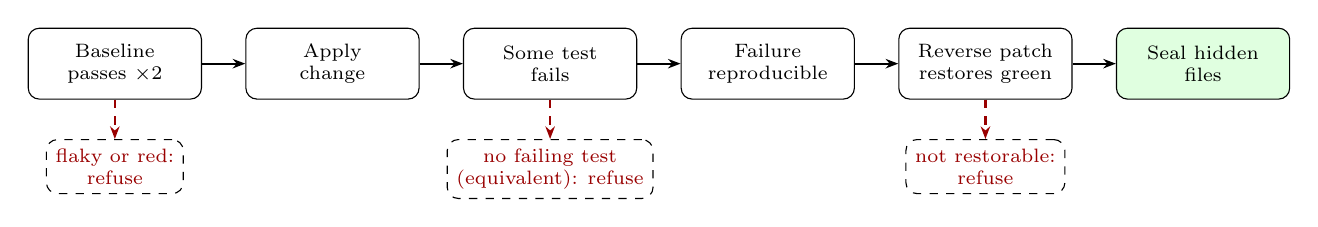
\begin{tikzpicture}[
  stp/.style={draw,rounded corners,align=center,minimum width=2.2cm,minimum height=0.9cm,font=\scriptsize},
  arr/.style={-{Stealth[length=1.6mm]},thick},
  rej/.style={draw,dashed,rounded corners,align=center,font=\scriptsize,text=red!60!black}]
\node[stp] (a) {Baseline\\passes $\times2$};
\node[stp,right=0.55cm of a] (b) {Apply\\change};
\node[stp,right=0.55cm of b] (c) {Some test\\fails};
\node[stp,right=0.55cm of c] (d) {Failure\\reproducible};
\node[stp,right=0.55cm of d] (e) {Reverse patch\\restores green};
\node[stp,right=0.55cm of e,fill=green!12] (f) {Seal hidden\\files};
\foreach \x/\y in {a/b,b/c,c/d,d/e,e/f} \draw[arr] (\x) -- (\y);
\node[rej,below=0.5cm of a] (ra) {flaky or red:\\refuse};
\node[rej,below=0.5cm of c] (rc) {no failing test\\(equivalent): refuse};
\node[rej,below=0.5cm of e] (re) {not restorable:\\refuse};
\draw[arr,dashed,red!60!black] (a) -- (ra);
\draw[arr,dashed,red!60!black] (c) -- (rc);
\draw[arr,dashed,red!60!black] (e) -- (re);
\end{tikzpicture}
\caption{Admission of a mutation-seeded repository task. Every refusal is counted by reason.}\label{fig:valid}
\end{figure}

\paragraph{Solving, recording and trajectory data.} The solver is a Sven coding worker with
file, search and shell tools, a tool-call budget and a repetition stop, started in a fresh
copy of the snapshot, with follow-up turns when the visible checks stay red.\cl{R03,PS01} The
recorded unit is the full trajectory; the verdict is produced outside the agent. Only
attempts whose patch passes and whose exposure audit is clean are eligible for
training;\cl{L06,L08} each assistant action becomes a training record conditioned on the prior
conversation and on the tool definitions the agent was offered, with system and user turns
carrying no loss, and compacted trajectories are excluded rather than repaired.\cl{D04,D05,D06,AU02}

\paragraph{Validity and leakage.} Four registered rules keep the exam honest. (i)~Families are
assigned to partitions by a stable hash before any rollout, and a family of the qualification
partition is never solved for data purposes.\cl{PR02,L07} (ii)~Hidden files are absent from the
solver's tree and are materialised only in the verifier's.\cl{V07} (iii)~An exposure audit fails
an attempt whose tool calls name a hidden path or whose outputs repeat a shingle of hidden
content, and exposed attempts and harness failures are withheld and counted in no
denominator.\cl{L06,L08,PR06} (iv)~The isolation level of every run is recorded; with
\code{none} the audit detects but cannot prevent, and a task whose soundness needs
isolation is not admitted.\cl{PR06,AU09} Whether a repository is in the base model's
pretraining data is not known; the base arm on the same exam bounds that effect without
removing it.

\paragraph{Units, arms and the paired exam.} The unit of analysis is the family, the file a
fault was seeded in for the authored repositories and the subsystem for real
ones.\cl{PR02} Tasks within a family are not independent, so no test treats them as such. The
base arm is the unmodified checkpoint in a pinned harness profile; the adapter arm is the same
checkpoint with the adapter attached; system prompt, tool schemas, budgets, seeds per
(task, attempt) and environment image are identical.\cl{PR03} A family is won by the adapter
when its resolved fraction is higher, lost when lower, and dropped when tied. The primary
decision is a one-sided exact sign test over the non-tied qualification families at
$\alpha=\alphalevel$, on the adapter served through Brain and driven by Sven; a result that is
not significant is \emph{not shown}, never equivalence.\cl{PR04,G03}

\begin{table}[t]
\centering\small
\input{generated/design_table}
\caption{The exact one-sided sign test at $\alpha=\alphalevel$: wins required and power if
each non-tied family is a win with the stated probability (a design calculation computed by
\code{scripts/build_data.py}, not a measurement).}\label{tab:design}
\end{table}

\paragraph{What the test can decide.} \Cref{tab:design} and \cref{fig:power} give the wins
needed and the power at assumed win probabilities: with fewer than five non-tied families no
decision is possible, \mDesignNOneFiveWins{} wins are needed at fifteen non-tied families
and \mDesignNTwoFiveWins{} at twenty-five, where the power at a win share of 0.8 is
\mDesignNTwoFivePowerEightZero{}.\cl{CP01,CP02} The registration therefore asks for about
twenty-five non-tied qualification families, fixed from the discordance of the baseline
experiment before any training, and labels a smaller comparison a pilot without changing the
rule.\cl{PR04}

\begin{figure}[t]
\centering
\begin{tikzpicture}
\begin{axis}[width=0.75\linewidth,height=5.2cm,xlabel={non-tied qualification families $n$},
  ylabel={power},ymin=0,ymax=1.02,xmin=2,xmax=40,legend pos=south east,
  legend style={font=\scriptsize},grid=major,
  every axis plot/.append style={thick}]
\addplot[blue,mark=none] table[col sep=comma,x=n,y=q70] {generated/power_curve.csv};
\addplot[red!70!black,mark=none,dashed] table[col sep=comma,x=n,y=q80] {generated/power_curve.csv};
\addplot[green!50!black,mark=none,dotted] table[col sep=comma,x=n,y=q90] {generated/power_curve.csv};
\legend{$P(\text{win})=0.7$,$P(\text{win})=0.8$,$P(\text{win})=0.9$}
\end{axis}
\end{tikzpicture}
\caption{Power of the exact one-sided sign test ($\alpha=\alphalevel$) against the number of
non-tied families. The sawtooth is the discreteness of the test.}\label{fig:power}
\end{figure}

\paragraph{Retention across rounds.} After each round $k$, the exam families of every earlier
round are solved again by the round-$k$ adapter and by its predecessor. Retention holds only if
the one-sided 95\% lower bound of the change in resolve rate (family-cluster bootstrap) exceeds
$-0.05$ absolute; a failed check refuses the candidate.\cl{PR05} The gate of
\cref{sec:gate} already holds each earlier release to the exam of its own run for repository
runs;\cl{G07} the open defects of \cref{sec:open} are why the registered check is stricter
than the gate's.

\paragraph{Controls and stop rules.} A gain must survive three controls, each a separate
training run on the same budget: training on trajectories regardless of verdict (does
verification matter), an adapter trained on a different repository (did it learn the tool
protocol rather than the repository), and no replay of earlier rounds.\cl{PR07} Registered
stop rules include dropping a task kind whose verifier false-pass rate exceeds 5\% and reporting
a development gain without a qualification gain as memorisation.\cl{PR08}

\paragraph{The code that exists.} \code{splinter practice} implements the stages of a
single-repository round from a revision to a gated release.\cl{PS01} Eight authored repository
families ship with the repository (\cref{tab:families}); a family's tests must pass five times
identically and its faults be caught before it is catalogued.\cl{PS02} What does not exist
yet is the benchmark verb that applies the partitions and the paired comparison of this section
to the base and the served adapter in one command; the experiments of \cref{sec:pending} wait on
it, and \cref{sec:replicate} marks each step as available now or planned.\cl{PL01}

% SPDX-License-Identifier: CC-BY-4.0
% Copyright (c) 2026 Martin Schröder <info@swedishembedded.com>

\section{The headline experiment and its replication: registered, not yet run}\label{sec:pending}

\paragraph{The claim this paper exists to establish.} Verified engineering-agent experience
can produce a sustained improvement in completion of previously unseen repository tasks,
under a controlled compute budget and without unacceptable loss of earlier capability.\cl{PR09}
\textbf{That claim is not yet measured.} No coding-task experiment has been run; this
section states exactly what will be run, what each outcome will mean, and where its numbers
will appear. Nothing in it is a result.

The experiments are registered in \code{prereg/coding-tasks.md}, dated 2026-10-16 and written
before any of their runs; they are kept apart from the first campaign's registration
(\code{prereg/protocol.md}), which is not amended. \Cref{tab:registered} lists them. Their
numbers will be read from \code{data/results.csv} by \code{scripts/build_data.py}; a row exists
only for a finished run, and the status column below changes by itself when one does.\cl{PL02}

\begin{table}[t]
\centering\small
\input{generated/registered_table}
\caption{The registered coding-task experiments. The status is derived from the rows of
\code{data/results.csv}.}\label{tab:registered}
\end{table}

\begin{description}
\item[CE1, the untrained agent.] The base agent's resolve rate on repository tasks, its failure
profile, its cost per resolved task and the discordance between two seeds of the same arm per
family, which sizes the qualification partition. No threshold; nothing is trained before it is
reported.\cl{PR10}
\item[CE4, the headline.] A LoRA adapter on Qwen3-8B trained only on verified trajectories from
development-partition families, compared with the base on the qualification partition by the
primary test of \cref{sec:protocol}, served through Brain and driven by Sven, with retention,
serve-verdict agreement and the three controls. The headline holds only if the sign test has
$p<0.05$, retention is not refused and agreement is within the serve check's tolerance; any
other outcome is reported as what it is, including ``no held-out improvement'' and
``memorisation''.\cl{PR11}
\item[CE6, the 27B model.] Ten stages from loading the exact model to comparing correctness,
tool-call validity and resources against the base, gated by training correctness and by
deployment agreement. The 27B is not used for a confirmatory query until both gates pass;
the training rate of \cref{sec:throughput} is reported as measured and no target is
registered.\cl{PR12}
\item[CE7, replication.] The unchanged CE1 and CE4 procedure on a second, independent
repository chosen by a rule fixed in advance (permissive licence, offline build, a suite of
bounded running time, no part of the pipeline tuned on it), with the cross cells that separate
learning a repository from learning the protocol. The headline counts as reproduced only if
both repositories pass the primary test independently.\cl{PR13}
\end{description}

\begin{table}[t]
\centering\small
\input{generated/results_table}
\caption{Paired outcomes over qualification-partition families (wins: the adapter resolves more
of the family than the base; losses: fewer), with the exact one-sided sign test. Every cell is
empty until its run exists; a cell is never filled with an estimate.}\label{tab:results}
\end{table}

\paragraph{What a failure would show.} An adapter that does not win, a gain that a different
repository's adapter or unverified trajectories match, a retention loss beyond the margin, or
a served adapter that disagrees with the in-process one are each stated outcomes of the
registration, and each is publishable as such. A development gain with no qualification gain
(sign test $p>0.2$) is reported as memorisation. If fewer than 25 non-tied families are
available the comparison is labelled a pilot and the rule is not loosened.\cl{PR08}

% SPDX-License-Identifier: CC-BY-4.0
% Copyright (c) 2026 Martin Schröder <info@swedishembedded.com>

\section{Replicating the result on another repository}\label{sec:replicate}

A result that only holds for the repositories it was developed on is a demonstration, not a
method. This section is the recipe for running the loop on a repository of one's own, with
the status of each step: \emph{available} means a command in the pinned revision does it and
the ledger checks the command line; \emph{planned} means the registration needs it and it
does not exist yet.\cl{PL01} It claims no outcome; the outcome of a replication is the
experiment CE7 of \cref{sec:pending}.

\subsection{Requirements on the repository}

\code{splinter practice} learns a codebase from its own tests: a git work tree or bare
repository, a revision git resolves to a commit, and a test suite that runs offline and is
green and stable on a clean copy of that revision. Splinter recognises a Python project with
a \code{tests} directory (run as \code{python3 -m unittest}) and a Cargo project (run with
\code{cargo test --offline}); any other suite is named with \code{--test-command}, and the files
tasks may change with repeated \code{--file}.\cl{PS01,PS04} The suite is run twice on a clean
copy first, and a red or flaky baseline stops the run before any model is loaded.\cl{PS01}
Isolation is \code{none} unless a container client and a digest-pinned image are configured;
a repository whose tests need isolation for soundness is not suitable on a host without
one.\cl{AU09}

\subsection{Task-family construction}

The protocol's unit is the family (\cref{sec:protocol}). \Cref{tab:families} shows what the
construction yields on the eight authored repositories that ship with Splinter: of several
hundred seeded faults per repository, those that do not build or that no test notices are
dropped, near-duplicates and truncated outputs are refused, and the rest are admitted.\cl{PS02}
For a new repository the steps are, in order:

\begin{enumerate}
\item \textbf{Check the environment} (available): \code{splinter doctor} confirms the state
root is writable with room to spare and the policy's weights fit the card.\cl{PS05}
\item \textbf{Generate and count the admitted tasks without a model} (available): run
\code{splinter practice REPO --rev REV --budget 1s --no-release --max-tasks N
--mutants-per-file M --test-command ...}; the \code{[tasks]} line states the admitted count
and the refusals by reason. This is the funnel of \cref{tab:families}, and it needs no model and
no GPU.\cl{PS03,PS06}
\item \textbf{Reserve the exam} (available): \code{--exam-families} sets families aside by a
stable hash of their names before any attempt, and \code{--exam-seed} is drawn, recorded and
refused if changed on a later run.\cl{PS06}
\item \textbf{Declare partitions and generations} (available for sealed families, planned for
the qualification partition): \code{splinter experiment check} validates a plan whose sealed
families are never trained on; a three-way split with a qualification partition queried once
is the registration's requirement and awaits the benchmark verb.\cl{PS07,PL01}
\item \textbf{Measure the untrained agent} (planned, CE1): the benchmark verb that runs the base
over development and qualification partitions with attempts per task fixed from a throughput
probe.\cl{PL01}
\item \textbf{Train and gate} (available for one round): \code{splinter practice REPO} solves the
non-exam tasks as an agent, keeps the attempts the hidden checks confirm, builds the
action-level SFT dataset, trains a LoRA candidate from the champion with earlier releases
replayed, and runs the release gate over the exam the run reserved; \code{--bf16-base},
\code{--steps}, \code{--rank} and \code{--max-block} bound the training to the card.\cl{PS01,PS06}
\item \textbf{Serve and roll back} (available): a release moves the alias and rewrites the
serving manifest, \code{brain serve --adapter-manifest} follows it, and \code{splinter rollback}
repoints it.\cl{X05,X06,PS08}
\end{enumerate}

\begin{table}[t]
\centering\small
\input{generated/families_table}
\caption{The eight authored repository families: language, tests, and tasks admitted by the
fault-seeding funnel (values read from the family catalogue at the pinned revision and
checked by the ledger).}\label{tab:families}
\end{table}

\subsection{What it costs}

Task generation costs CPU time only: no model is loaded and no GPU is used.\cl{PS03} Training
cost on a 27B model is the token count over the measured rate; at the \mThrNfFourEightOneNineTwoTokensPerS{}~tokens/s of the
probe of \cref{sec:throughput} one million trained tokens take \mThrHoursPerMillionTokens{}~h
of card time.\cl{M38,C12} The remaining terms of the cost of one verified outcome, wall time and
tokens per attempt and attempts per resolved task, are measured by CE1 and are not known
today; they are the reason CE1 precedes any training. A replication should budget by first
running step 2, then CE1 on a small number of families, and only then committing card time.

\subsection{What to report}

For a replication to count it must report, for the new repository, the same quantities as
\cref{sec:pending}: the admission funnel by reason, the baseline resolve rate with its
interval, the paired sign-test counts on the qualification partition, the retention check,
the isolation level and the three repository commits. Counts that disagree with ours are as
informative as ones that agree.\cl{PR13}

% SPDX-License-Identifier: CC-BY-4.0
% Copyright (c) 2026 Martin Schröder <info@swedishembedded.com>

\section{Limitations}\label{sec:limitations}

The structure claims show that definitions, constants, tests and messages exist at the pinned
commits; they do not show that the code behaves accordingly. Behaviour is established only by
the experiments, which are pilots: one run each per setting, one generator family, small
corpora, 30 facts per generation, one policy size per run. The training settings of E2 were
chosen on two earlier pilots with other seeds, not on the registered run's own measurement, but
they were chosen by hand and no search over them was made.

The registered E2/E3 criterion (a release with a significant gain, then retention and rollback) was not
met: every candidate of the 0.6B policy passed the improvement and retention checks and was refused by the
anchor check, whose bound of 0.02 over 40 questions (0.025 per question) allows no lost answer. One
post hoc run with a 1.7B policy released its first candidate; its second candidate was refused, so the
alias move after a second release, retention against an earlier release as the gate measures it and the rollback
to a first release are described from the code (\cref{sec:gate}) and are not demonstrated end to end here;
the one rollback attempted was refused because the release had no predecessor. In one run the serve check
could not start its server and is not measured. The gate's retention check held the champion to held-out tasks that,
for a facts campaign, are facts it never taught, so it passed while the candidate forgot taught facts
(\cref{sec:e2}); we measured that forgetting on independent probes. The 1.7B result is a single post hoc run.
We did not test a larger anchor suite or other settings that might keep the anchor at 0.6B beyond the two
reported. The facts are numbers, which may be why they leak into numeric answers elsewhere; a
domain of non-numeric facts is not measured.

The held-out families of a run are facts the policy is never taught, a few of the 30 facts of a
generation, and the teacher's answer was not verified for a further share of them
(\cref{sec:defects}); the facts measured in the probes include both, so the counts of facts answered
are lower bounds of what the trained records taught. Probes are graded by numbers appearing in the
answer; a different grader was not compared. The experiments ran on binaries built from the commits
of \cref{sec:repro}, which differ between the first and second wave and, for the repaired-verifier
rerun, from the registered run's; each result names its wave. The training qualification of the 27B
model used random weights for the long sequences and a handful of examples for the real checkpoint;
it shows that steps fit and run, not that the adapter changes generation, and no sequence longer
than 16384 tokens was run.

The cause of the generator's missing subjects is localised, not resolved: the rule is not at fault
beyond the markup case, the generator at two sizes names a subject its question omits, and a changed
brief was not tested. Corpus expansion beyond the first pass (variants, retention queue,
rehearsal, claims) is described from the code; variants and rehearsal were exercised as stage
counts and as a post hoc setting, and none of the mechanisms was evaluated for the value it adds.

\paragraph{The coding-task experiment.} It is not measured. Everything said about it in
\cref{sec:protocol,sec:pending,sec:replicate} is a registered rule or a statement about code; the
sign-test table is a design calculation. The registration fixes one model size for the first
training result (Qwen3-8B, because training, saving and serving an adapter work end to end for
it), one agent harness, and runs with process isolation \code{none} on the node, so the exposure
audit detects but cannot prevent a solver reading hidden files (\cref{sec:audit}).\cl{AU09} Mutation-seeded
tasks test whether a model can undo a synthetic fault, not whether it can debug a historical one;
tasks from repository history are registered as a source, not yet built.\cl{PR10} A family is the file a
fault was seeded in for the authored repositories, so clusters are files, not subsystems.\cl{PR02}
An exam of one repository may hold too few non-tied families to decide, and the registration
labels such a comparison a pilot instead of changing the rule. The base model may have seen
public repositories in pretraining; the paired base arm bounds that effect, it does not remove it.
Agent rollouts of realistic length make training cost unmeasured for the 8B model; the only
training rate measured here is that of the 27B architecture (\cref{sec:throughput}), on one card,
one revision and one sequence length.

\paragraph{Open defects.} The retention check is blind to taught facts, the default anchor bound
refuses on one net lost answer in a small suite, a workspace pass is an exit status, and the
practice gate has no canaries (\cref{sec:open}). The first campaign was not rerun with the
repairs that exist, so its reported outcome describes the build of its time.

\input{generated/limitations}

% SPDX-License-Identifier: CC-BY-4.0
% Copyright (c) 2026 Martin Schröder <info@swedishembedded.com>

\section{Reproducibility}\label{sec:repro}

\paragraph{Verification.} \code{make -C papers/splinter-brain-sven-flywheel verify} first runs the
specification of the pin rule, then re-runs every structure check against the commits in
\code{data/commits.json}, then \code{scripts/build_data.py --check}, which resolves each measured,
computed, registered and planned claim to its record, requires the claim text to contain the value,
and requires every ledger row to be cited in the text and every citation to be in the ledger.
The ledger holds \mLedgerClaims{} claims, \mLedgerStructure{} of them structure claims backed by
\mLedgerChecks{} checks. A pin must be contained in a remote-tracking ref of its repository, so a
fresh clone of the three remotes reproduces the result; the verification was run on such a clone
of the remotes, with the sibling repositories given by \code{--sven} and \code{--brain}. The
splinter pin is the reachable twin of an earlier pin that no branch contained.
\code{make check} includes this verification as \code{check/papers}. The bibliography entries
were checked against the archive's abstract pages on 2026-10-16.

\paragraph{Experiments.} The exact commands are in \code{scripts/run_experiments.sh}; raw records
are copied into \code{data/runs} by \code{scripts/archive_run.sh} with this machine's paths replaced.
The first wave ran a Splinter binary built from the main checkout at the time (Splinter
\code{ce42a55} plus uncommitted repairs, Sven \code{02adbda7}, Brain \code{dc50b7cc}; binary sha256
prefix \code{f91620c5}); its records are in \code{data/runs/e1} and \code{data/runs/e2}. The second wave
ran binaries of Splinter's main branch at the commit before this paper's change plus the repairs of
\cref{sec:defects} in the order listed there (the E1 reruns and the registered E2 run the first three
repairs and the serve-bank repair; the repaired-verifier rerun and E2d also the verifier repair), against Sven
at its local main \code{ebd169a2} and a Brain release binary built from \code{f9f909f7}
(\code{--features brain/study}), with a CUDA 13 toolkit on the card's host. Splinter's models run in its process
(Vulkan adapter line in the logs); \code{brain serve} in the gate's serve check ran with the CUDA backend.
Models: Qwen3-0.6B or Qwen3-1.7B (policy), Qwen3-4B (generator, teacher; Qwen3-8B in E1c), on a shared NVIDIA GH200, so wall times are not
comparable between runs. The seeds drawn by the runs are in the raw records (denoise seed in
\code{tasks.json}, fact seed in \code{build.json}, training seeds in each \code{learn-g*.stderr}). The protocol was
fixed before the runs and extended before each later one (\code{prereg/protocol.md}); the pilots that chose the
training flags are described there and are not part of any claim. Deviations: E1 ran without a time limit; the registered E2 success
criterion was not met; a repaired run, a post hoc run and a post hoc E1 variant are reported beside it and labelled;
the E2d run was assembled from three invocations of the same script
(\code{run} until its first served probe failed on an authentication bug of the script, repaired in \code{finish}, whose
served probes were stopped under load; the rollback of its first release; and \code{second\_generation.py}, the second \code{learn} on a copy
of its state taken before the rollback), all on the state
the first produced, nothing retried.

\paragraph{Training qualification and throughput.} The logs in \code{data/runs/qual} are Brain's
qualification logs at commit \mEFourCommit{}; each log's header records its command. They contain
only the runs that finished; runs that were planned and not run are not reported as results. The
throughput probe in \code{data/runs/throughput} is a copy of a log kept with the correction plan;
its header says what the roadmap records about its command and revision, and that the log itself
carries no commit.

\paragraph{Coding-task experiments.} None has been run. The registration is
\code{prereg/coding-tasks.md}; results will be rows of \code{data/results.csv} with the commands,
commits, harness profile and seeds of the run, and the tables of \cref{sec:pending} are generated
from them.

\paragraph{Build.} \code{make papers/splinter-brain-sven-flywheel/pdf} builds the paper to
\code{target/papers}; the tables and numbers are generated from \code{data/runs} into the
build directory.


\bibliographystyle{plainnat}
\bibliography{references}

\end{document}
